% !TeX program = pdflatex
% =============================================================
% Public Economics -- Lecture 7
% Externalities: Problems and Solutions
% Based on: Saez, E. "Econ 131" (UC Berkeley), Lecture Notes on Externalities
%           Gruber, J. "Public Finance and Public Policy", Ch. 5
%           (5.1-5.5, Externalities: Problems and Solutions)
%           Gruber, J. "Public Finance and Public Policy", S6.1
%           (The Role of Economics in Environmental Regulation: The Case of Particulates)
% =============================================================
\documentclass[11pt,aspectratio=169]{beamer}

\usetheme{metropolis}
\usepackage[utf8]{inputenc}
\usepackage[T1]{fontenc}
\usepackage{lmodern}
\usepackage{booktabs}
\usepackage{array}
\usepackage{textcomp}
\usepackage{siunitx}
\usepackage{tikz}
\usepackage{pgfplots}
\pgfplotsset{compat=1.18}
\usetikzlibrary{positioning,arrows.meta,calc}

% ----------------------------------------------------------------
% Colors: WU Vienna blue as primary accent
% ----------------------------------------------------------------
\definecolor{wublue}{HTML}{003D7C}
\definecolor{wulight}{HTML}{4F8FC4}
\definecolor{wugray}{HTML}{5C6670}
\definecolor{wured}{HTML}{B0202E}
\definecolor{wugreen}{HTML}{4C8C6B}
\definecolor{wuyellow}{HTML}{D9A441}
\setbeamercolor{palette primary}{bg=wublue,fg=white}
\setbeamercolor{frametitle}{bg=wublue,fg=white}
\setbeamercolor{progress bar}{fg=wublue,bg=wulight!30}
\setbeamercolor{alerted text}{fg=wured}

\setbeamertemplate{frame footer}{Externalities}
\setbeamertemplate{footline}[frame number]

\title{Public Economics}
\subtitle{Lecture 7 \(\cdot\) Externalities: Problems and Solutions}
\author{Shushanik Margaryan}
\institute{WU Vienna University of Economics and Business}
\date{Winter Term}

% Source note command for footnote-style citations on data slides
\newcommand{\srcnote}[1]{{\footnotesize\color{wugray}Source: #1}}

\begin{document}

% =============================================================
\begin{frame}
  \titlepage
\end{frame}

\begin{frame}{Today's Questions}
  \begin{itemize}
    \item When does one person's or firm's action make someone else better or worse off \emph{without} going through a price --- and why does the market then get the quantity wrong?
    \item Can private bargaining ever fix this on its own, and when does it predictably fail?
    \item What are the government's main tools --- taxes, subsidies, regulation, tradable permits --- and when is each the right one?
  \end{itemize}
  \vspace{1em}
  \begin{block}{Based on}
    Saez, E., \emph{Econ 131} lecture notes (UC Berkeley); Gruber, J. \emph{Public Finance and Public Policy}, Ch.\ 5 (\S5.1--5.5) and \S6.1.
  \end{block}
\end{frame}

% =============================================================
\begin{frame}{Outline}
  \tableofcontents
\end{frame}

% =============================================================
\section{5.1 Externality Theory}

\begin{frame}{What Is an Externality?}
  \begin{block}{Market failure}
    A problem that violates an assumption of the First Welfare Theorem, so the market economy no longer delivers an efficient outcome.
  \end{block}
  \begin{block}{Externality}
    Arises whenever the actions of one economic agent \textbf{directly} affect another agent \emph{outside the market mechanism}.
  \end{block}
  \begin{itemize}
    \item \textbf{Externality:} a steel plant that dumps sludge into a river used by fishers.
    \item \textbf{Not an externality:} a steel plant buys more electricity and bids up the price for other customers --- that effect runs entirely \emph{through} the market.
    \item The single biggest externality on the planet: carbon-intensive growth since the 19th century, driving climate change.
  \end{itemize}
\end{frame}

\begin{frame}{Application: The Externality of an SUV}
  Driving a large, gas-powered SUV generates at least four distinct negative externalities on other people:
  \begin{enumerate}
    \item \textbf{Environmental:} carbon emissions contribute to global warming.
    \item \textbf{Infrastructure:} heavier vehicles wear down public roads faster.
    \item \textbf{Safety:} the odds of a fatal accident rise for whoever is hit by a bigger car.
    \item \textbf{Congestion:} one more car on the road adds to everyone else's travel time.
  \end{enumerate}
  \vspace{0.3em}
  None of these costs shows up on the sticker price --- the buyer never has to weigh them.
\end{frame}

\begin{frame}{Quiz: Which Is \emph{Not} a Negative Externality?}
  \begin{block}{Question}
    Which of the following is \textbf{not} a negative externality?
  \end{block}
  \begin{enumerate}
    \item[A.] Cigarette smoking that damages your \emph{future} health.
    \item[B.] Texting while driving, which increases accident risk.
    \item[C.] Pesticide runoff from farms that pollutes land and water.
    \item[D.] Noise from a construction project.
    \item[E.] All are negative externalities.
  \end{enumerate}
  \vspace{0.4em}
  \small \emph{Hint:} an externality must fall on \textbf{someone else}. Damage to your own future health is a private cost you already bear --- not an externality.
\end{frame}

\begin{frame}{Negative Production Externalities}
  \begin{block}{Negative production externality}
    A firm's production reduces others' well-being, and the firm is not made to pay for it.
  \end{block}
  \begin{itemize}
    \item \textbf{Private marginal cost (PMC):} the direct cost to the producer of one more unit $=$ the supply curve.
    \item \textbf{Marginal damage (MD):} the extra cost imposed on others that the producer does \emph{not} pay.
    \item \textbf{Social marginal cost} \(SMC = PMC + MD\).
  \end{itemize}
  \vspace{0.4em}
  \textbf{Example:} a coal plant's private cost curve reflects fuel and labor --- not the CO\textsubscript{2} it emits.
\end{frame}

\begin{frame}{Diagram: Negative Production Externality}
  \begin{center}
  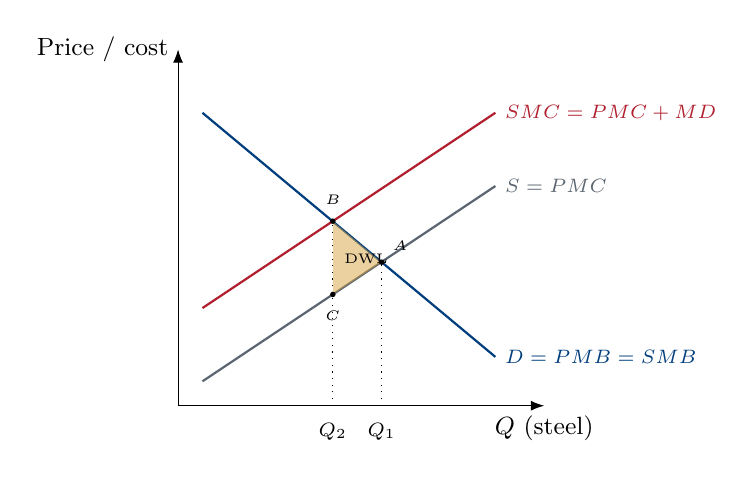
\begin{tikzpicture}[scale=0.62]
    \draw[-{Latex}] (0,0) -- (7.5,0) node[below, font=\small]{$Q$ (steel)};
    \draw[-{Latex}] (0,0) -- (0,7.3) node[left, font=\small]{Price / cost};
    \draw[wugray, thick] (0.5,0.5) -- (6.5,4.5);
    \node[right, font=\scriptsize, wugray] at (6.5,4.5) {$S=PMC$};
    \draw[wured, thick] (0.5,2.0) -- (6.5,6.0);
    \node[right, font=\scriptsize, wured] at (6.5,6.0) {$SMC=PMC+MD$};
    \draw[wublue, thick] (0.5,6) -- (6.5,1);
    \node[right, font=\scriptsize, wublue] at (6.5,1) {$D=PMB=SMB$};
    \fill[wuyellow, opacity=0.5] (4.17,2.94) -- (3.17,3.78) -- (3.17,2.28) -- cycle;
    \node[font=\tiny] at (3.85,3.0) {DWL};
    \fill (4.17,2.94) circle (1.6pt); \node[above right, font=\tiny] at (4.2,2.98) {$A$};
    \fill (3.17,3.78) circle (1.6pt); \node[above, font=\tiny] at (3.17,3.92) {$B$};
    \fill (3.17,2.28) circle (1.6pt); \node[below, font=\tiny] at (3.17,2.15) {$C$};
    \draw[dotted] (4.17,0) -- (4.17,2.94);
    \draw[dotted] (3.17,0) -- (3.17,3.78);
    \node[below, font=\scriptsize] at (4.17,-0.15) {$Q_1$};
    \node[below, font=\scriptsize] at (3.17,-0.15) {$Q_2$};
  \end{tikzpicture}
  \end{center}
  \footnotesize The free market settles at $A$, where $PMC=PMB$, producing $Q_1$. The social optimum is $B$, where $SMC=SMB$, at the lower quantity $Q_2$. Triangle $ABC$ is the deadweight loss from \textbf{overproduction}.
\end{frame}

\begin{frame}{Negative Consumption Externalities}
  \begin{block}{Negative consumption externality}
    An individual's consumption reduces others' well-being, and the individual is not made to pay for it.
  \end{block}
  \begin{itemize}
    \item \textbf{Private marginal benefit (PMB):} the direct benefit to the consumer of one more unit $=$ the demand curve.
    \item \textbf{Social marginal benefit} \(SMB = PMB - MD\).
  \end{itemize}
  \vspace{0.4em}
  \textbf{Example:} gasoline that powers a car contributes to global warming --- a cost the driver enjoys the benefit of driving without paying.
\end{frame}

\begin{frame}{Diagram: Negative Consumption Externality}
  \begin{center}
  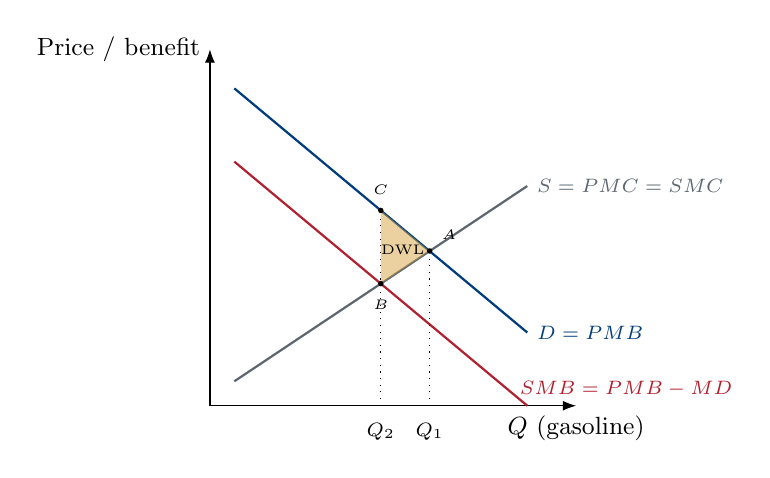
\begin{tikzpicture}[scale=0.62]
    \draw[-{Latex}] (0,0) -- (7.5,0) node[below, font=\small]{$Q$ (gasoline)};
    \draw[-{Latex}] (0,0) -- (0,7.3) node[left, font=\small]{Price / benefit};
    \draw[wugray, thick] (0.5,0.5) -- (6.5,4.5);
    \node[right, font=\scriptsize, wugray] at (6.5,4.5) {$S=PMC=SMC$};
    \draw[wublue, thick] (0.5,6.5) -- (6.5,1.5);
    \node[right, font=\scriptsize, wublue] at (6.5,1.5) {$D=PMB$};
    \draw[wured, thick] (0.5,5.0) -- (6.5,0.0);
    \node[right, font=\scriptsize, wured] at (6.15,0.35) {$SMB=PMB-MD$};
    \fill[wuyellow, opacity=0.5] (4.5,3.17) -- (3.5,2.5) -- (3.5,4.0) -- cycle;
    \node[font=\tiny] at (3.95,3.2) {DWL};
    \fill (4.5,3.17) circle (1.6pt); \node[above right, font=\tiny] at (4.55,3.2) {$A$};
    \fill (3.5,2.5) circle (1.6pt); \node[below, font=\tiny] at (3.5,2.37) {$B$};
    \fill (3.5,4.0) circle (1.6pt); \node[above, font=\tiny] at (3.5,4.13) {$C$};
    \draw[dotted] (4.5,0) -- (4.5,3.17);
    \draw[dotted] (3.5,0) -- (3.5,4.0);
    \node[below, font=\scriptsize] at (4.5,-0.15) {$Q_1$};
    \node[below, font=\scriptsize] at (3.5,-0.15) {$Q_2$};
  \end{tikzpicture}
  \end{center}
  \footnotesize The market settles where $S=PMB$ (point $A$, quantity $Q_1$); the optimum is where $S=SMB$ (point $B$, quantity $Q_2 < Q_1$). Same story as before: \textbf{overconsumption} and a deadweight loss.
\end{frame}

\begin{frame}{Positive Externalities}
  \begin{columns}[T]
    \begin{column}{0.5\textwidth}
      \textbf{Positive production externality}\\
      \small A firm's production raises others' well-being without compensation.\\
      $SMC = PMC - MB$\\[0.4em]
      \emph{Example:} beehives that pollinate neighboring farms' crops.
    \end{column}
    \begin{column}{0.5\textwidth}
      \textbf{Positive consumption externality}\\
      \small An individual's consumption raises others' well-being without compensation.\\
      $SMB = PMB + MB$\\[0.4em]
      \emph{Example:} a beautiful private garden that passers-by enjoy.
    \end{column}
  \end{columns}
  \vspace{0.8em}
  \textbf{The two biggest positive externalities in the economy:}
  \begin{itemize}
    \item \textbf{Technology spillovers:} better production processes get copied and drive long-run growth.
    \item \textbf{Education and research:} fundamental knowledge spills over into production (NIH, NSF; Stanford/Berkeley and Silicon Valley).
  \end{itemize}
\end{frame}

\begin{frame}{Diagram: Positive Production Externality (R\&D)}
  \begin{center}
  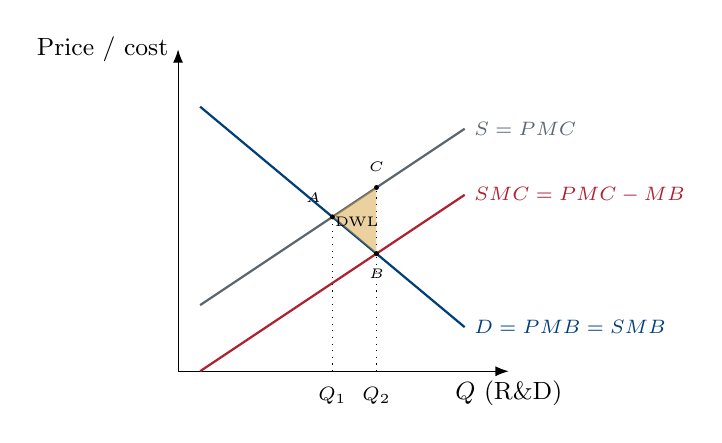
\begin{tikzpicture}[scale=0.56]
    \draw[-{Latex}] (0,0) -- (7.5,0) node[below, font=\small]{$Q$ (R\&D)};
    \draw[-{Latex}] (0,0) -- (0,7.3) node[left, font=\small]{Price / cost};
    \draw[wugray, thick] (0.5,1.5) -- (6.5,5.5);
    \node[right, font=\scriptsize, wugray] at (6.5,5.5) {$S=PMC$};
    \draw[wured, thick] (0.5,0.0) -- (6.5,4.0);
    \node[right, font=\scriptsize, wured] at (6.5,4.0) {$SMC=PMC-MB$};
    \draw[wublue, thick] (0.5,6) -- (6.5,1);
    \node[right, font=\scriptsize, wublue] at (6.5,1) {$D=PMB=SMB$};
    \fill[wuyellow, opacity=0.5] (3.5,3.5) -- (4.5,2.667) -- (4.5,4.167) -- cycle;
    \node[font=\tiny] at (4.05,3.4) {DWL};
    \fill (3.5,3.5) circle (1.6pt); \node[above left, font=\tiny] at (3.45,3.6) {$A$};
    \fill (4.5,2.667) circle (1.6pt); \node[below, font=\tiny] at (4.5,2.53) {$B$};
    \fill (4.5,4.167) circle (1.6pt); \node[above, font=\tiny] at (4.5,4.3) {$C$};
    \draw[dotted] (3.5,0) -- (3.5,3.5);
    \draw[dotted] (4.5,0) -- (4.5,4.167);
    \node[below, font=\scriptsize] at (3.5,-0.15) {$Q_1$};
    \node[below, font=\scriptsize] at (4.5,-0.15) {$Q_2$};
  \end{tikzpicture}
  \end{center}
  \footnotesize The market settles at $A$ ($Q_1$, where $PMC=D$); the optimum $B$ requires \emph{more} R\&D ($Q_2>Q_1$, where $SMC=D$). Positive externalities cause \textbf{underprovision}.\\
  \srcnote{Bloom, Schankerman \& Van Reenen (2013): private return to R\&D $\approx$21\%, social return $\approx$58\%.}
\end{frame}

\begin{frame}{Why the Market Gets It Wrong}
  A competitive market sets quantity where \(PMB = PMC\). The efficient (social) optimum requires \(SMB = SMC\). Whenever an externality drives a wedge between private and social curves, the two conditions diverge:
  \begin{center}
  \begin{tabular}{@{}lcc@{}}
    \toprule
    \textbf{Externality} & \textbf{Direction of gap} & \textbf{Market outcome} \\
    \midrule
    Negative production & $SMC>PMC$ & Overproduction \\
    Positive production & $SMC<PMC$ & Underproduction \\
    Negative consumption & $SMB<PMB$ & Overconsumption \\
    Positive consumption & $SMB>PMB$ & Underconsumption \\
    \bottomrule
  \end{tabular}
  \end{center}
  \vspace{0.5em}
  In every case, the First Welfare Theorem fails --- and government intervention is \emph{potentially} justified.
\end{frame}

% =============================================================
\section{5.2 The Coase Theorem}

\begin{frame}{Are Externalities Really Outside the Market?}
  Ronald Coase (Nobel laureate, Chicago) posed a provocative question: are externalities \emph{really} beyond the reach of private bargaining?
  \begin{block}{Internalizing the externality}
    When private negotiation or government action makes the price a party faces fully reflect the external costs or benefits of that party's actions.
  \end{block}
  If the answer is often ``yes,'' many externalities may not need government intervention at all.
\end{frame}

\begin{frame}{The Coase Theorem}
  \begin{block}{Coase Theorem, Part I}
    With well-defined property rights and costless bargaining, negotiation between the party creating an externality and the party affected by it can achieve the socially optimal quantity.
  \end{block}
  \begin{block}{Coase Theorem, Part II}
    The efficient quantity does not depend on \emph{which} party is assigned the property rights --- only that \emph{someone} is.
  \end{block}
\end{frame}

\begin{frame}{Coase Theorem: The Steel Plant and the Swimmers}
  A steel plant pollutes a river enjoyed by swimmers. Left alone, there is too much pollution.
  \begin{itemize}
    \item \textbf{If swimmers own the river:} they can charge the plant for polluting --- and will charge exactly the marginal damage (\(MD\)) per unit. Charge above \(MD\) and swimmers would rather sell one more unit of pollution than suffer it; the price settles at \(MD\).
    \item \textbf{If the plant owns the river:} it can charge swimmers to reduce its pollution --- and will again charge \(MD\) per unit of reduction.
  \end{itemize}
  \vspace{0.4em}
  \textbf{Either way, the final level of pollution is the same} --- exactly Part II of the theorem.
\end{frame}

\begin{frame}{Problems with Coasian Solutions: Assignment}
  In practice, Coasian bargaining is unlikely to resolve most externalities that cause real market failures.
  \begin{block}{1. The assignment problem}
    Assigning property rights is hard when an externality touches many agents at once --- think of global warming, where responsibility and damage are both diffuse.
  \end{block}
  \small Coasian solutions work best for \textbf{small, localized} externalities: beehive pollination has become an ordinary business transaction, not an external side-effect, precisely because the parties are few and identifiable. Large, global externalities involving countless firms and people are a different story.
\end{frame}

\begin{frame}{Problems with Coasian Solutions: Negotiating Costs}
  \begin{block}{2. Transaction costs and negotiating problems}
    Negotiating is costly --- especially with large numbers of people on one or both sides.
  \end{block}
  \small This problem is amplified for something like global warming, where the potentially divergent interests of billions of people on one side of the bargain must somehow be aggregated before any negotiation can even start.
  \vspace{0.6em}

  \normalsize
  \begin{alertblock}{Bottom line}
    Coase's insight is a genuine defense of the competitive model against small-scale externalities. But for large-scale, global externalities, only a government can aggregate the interests of everyone affected --- private bargaining alone will not get there.
  \end{alertblock}
\end{frame}

% =============================================================
\section{5.3 Public-Sector Remedies}

\begin{frame}{Public-Sector Remedies: Three Tools}
  When Coasian bargaining fails, policy makers reach for one of three instruments:
  \begin{enumerate}
    \item \textbf{Quantity regulation:} limit or ban the externality-producing activity directly (e.g., the 1990s ban on ozone-depleting CFCs).
    \item \textbf{Corrective (Pigouvian) taxation or subsidy:} a per-unit tax or subsidy equal to the marginal damage or benefit (e.g., a carbon tax).
    \item \textbf{Tradable permits:} combine 1 and 2 --- cap the total quantity, but let firms trade the right to pollute (cap-and-trade).
  \end{enumerate}
  \vspace{0.4em}
  \small The key advantage economists see in price-based tools (2 and 3): the price of emissions ends up the \emph{same for everyone}, which is what efficiency requires.
\end{frame}

\begin{frame}{Corrective Taxation}
  Taxing the polluter an amount \(t = MD\) per unit raises \(PMC\) up to \(SMC\) --- exactly what a swimmer-owned river would have charged under Coase. Revisit the negative-production diagram: a \$100-per-unit tax shifts $PMC_1$ up to $PMC_2 = SMC$, and the market moves itself from $A$ (quantity $Q_1$) to the efficient point $B$ (quantity $Q_2$).
  \begin{itemize}
    \item This is called \textbf{Pigouvian taxation}, after economist A.\ C.\ Pigou.
    \item Unlike Coase, it works \emph{without} needing anyone to negotiate --- the government sets the price once, for everyone.
  \end{itemize}
\end{frame}

\begin{frame}{Application: Congestion Pricing}
  Traffic congestion is a textbook negative externality: each additional driver slows down, and pollutes for, everyone else. Congestion costs the US over \$150 billion a year.
  \begin{itemize}
    \item \textbf{London (2003):} $\approx$\pounds15--21 daily charge to enter an 8-square-mile zone; private cars entering fell by 39\%.
    \item \textbf{Stockholm:} a variable charge (up to \$12.50) that rises with the size of the externality at that time and place; children's asthma-related hospital visits fell $\approx$15\% per unit of pollution reduced.
    \item \textbf{New York City (2019):} the first US city to adopt congestion pricing --- but implementation has been politically fraught.
  \end{itemize}
  \small Success depends on offering alternatives: London added 300 extra buses the day its charge began.
\end{frame}

\begin{frame}{Subsidies for Positive Externalities}
  The mirror image of a corrective tax: pay a subsidy \(s = MB\) per unit to push \(PMC\) down to \(SMC\), moving production from the underprovided market quantity up toward the efficient one.
  \begin{itemize}
    \item \textbf{R\&D tax credits:} subsidize innovation --- though rarely tied precisely to the size of the spillover.
    \item \textbf{Charitable-giving tax deduction:} subsidizes an activity that benefits others, again without measuring the externality directly.
    \item \textbf{Vaccination:} a classic positive consumption externality --- your shot protects people who aren't yet vaccinated. Operation Warp Speed combined ``push'' grants (\$12.4B for vaccine R\&D) with ``pull'' advance-purchase guarantees, cutting typical vaccine development time from 10--15 years to seven months.
  \end{itemize}
\end{frame}

\begin{frame}{Quiz: The Coffee Pesticide}
  \begin{block}{Question}
    A new pesticide helps grow coffee more cheaply but is toxic. Marginal damage is \$10/unit where it's used (poor country), but would be \$100/unit in the US. What is the correct remedy?
  \end{block}
  \begin{enumerate}
    \item[A.] A \$10 tax per unit.
    \item[B.] A \$100 tax per unit.
    \item[C.] Nothing.
    \item[D.] The pesticide should be entirely prohibited.
  \end{enumerate}
  \vspace{0.4em}
  \small \emph{Hint:} the corrective tax equals the \textbf{marginal damage where the externality actually occurs} --- not damage estimated somewhere else.
\end{frame}

\begin{frame}{Quiz: Inelastic Demand for Gasoline}
  \begin{block}{Question}
    Gasoline generates a climate-change marginal external cost of \$2/gallon. Suppose gasoline consumption is completely \textbf{inelastic} to price. What is the correct remedy for efficiency?
  \end{block}
  \begin{enumerate}
    \item[A.] A \$2 tax per gallon.
    \item[B.] Nothing.
    \item[C.] Either A or B.
    \item[D.] Phase out gas cars.
  \end{enumerate}
  \vspace{0.4em}
  \small \emph{Hint:} if quantity can't respond to price, does the tax change behavior --- or does it still matter for who pays the external cost?
\end{frame}

\begin{frame}{Regulation in Practice}
  \textbf{The single most common real-world response to externalities is not a tax --- it's regulation:} products or actions that cause harm are simply forbidden by law (toxic pollutants, dangerous consumer goods, littering, speeding).
  \begin{itemize}
    \item A fine is economically equivalent to a tax --- but psychologically and socially very different: the goal is to \emph{prohibit}, not to price, the externality.
    \item Emissions limits (e.g., California's smog check for gas cars) are a quantity constraint on individual behavior.
  \end{itemize}
  \begin{alertblock}{The economist's objection}
    Reduction is cheap in some settings and expensive in others: electric cars already exist, electric planes do not. A single CO\textsubscript{2} allowance applied uniformly could cripple high-value aviation while barely touching easy-to-decarbonize sectors.
  \end{alertblock}
\end{frame}

\begin{frame}{Cap-and-Trade: Taxes and Regulation Combined}
  \textbf{Emission permits and trading:} polluters are issued permits and allowed to trade them. If the total number of permits is set so that the resulting price equals \(MD\), the outcome is efficient --- and the price is automatically the \emph{same for every firm}.
  \begin{itemize}
    \item Used historically as a \textbf{transition tool}: SO\textsubscript{2} (acid rain) and CFCs (ozone) were both phased out gradually through shrinking, tradable allowances rather than an immediate ban --- giving industry time to develop substitutes.
  \end{itemize}
\end{frame}

\begin{frame}{Corrective Taxes vs.\ Tradable Permits}
  Two key differences between a carbon tax and cap-and-trade for CO\textsubscript{2}:
  \begin{enumerate}
    \item \textbf{Initial allocation of permits.} Selling permits is economically equivalent to a tax. \emph{Giving} them away to incumbent polluters is like a tax \emph{plus} a large transfer to those firms.
    \item \textbf{Uncertainty about marginal costs.} A tax fixes the \emph{price} of pollution but leaves the resulting \emph{quantity} uncertain; a cap fixes the \emph{quantity} but leaves the price uncertain.
  \end{enumerate}
  \vspace{0.5em}
  \begin{block}{Rule of thumb}
    \textbf{Taxes} are preferable when the marginal-damage curve is \textbf{flat} (getting the quantity exactly right barely matters). \textbf{Tradable permits} are preferable when marginal damage is \textbf{steep} (getting the quantity right matters a great deal).
  \end{block}
\end{frame}

\begin{frame}{Why Steepness of Marginal Damage Matters}
  \begin{columns}[T]
    \begin{column}{0.5\textwidth}
      \centering \textbf{Flat MD (e.g., climate change)}\\[0.2em]
      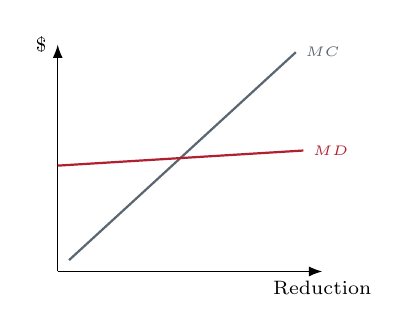
\begin{tikzpicture}[scale=0.48]
        \draw[-{Latex}] (0,0) -- (7,0) node[below, font=\scriptsize]{Reduction};
        \draw[-{Latex}] (0,0) -- (0,6) node[left, font=\scriptsize]{\$};
        \draw[wugray, thick] (0.3,0.3) -- (6.3,5.8);
        \draw[wured, thick] (0,2.8) -- (6.5,3.2);
        \node[right, font=\tiny, wugray] at (6.3,5.8) {$MC$};
        \node[right, font=\tiny, wured] at (6.5,3.2) {$MD$};
      \end{tikzpicture}\\[0.3em]
      \small One country's emissions barely move total accumulated CO\textsubscript{2} --- a small quantity miss costs almost nothing, so a stable, predictable \textbf{tax} is efficient.
    \end{column}
    \begin{column}{0.5\textwidth}
      \centering \textbf{Steep MD (e.g., forest fires)}\\[0.2em]
      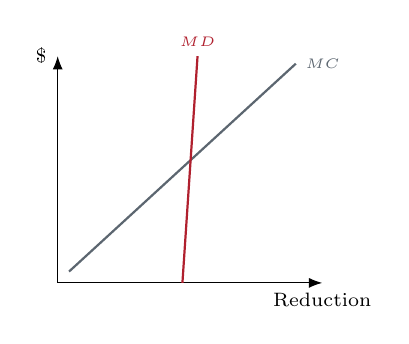
\begin{tikzpicture}[scale=0.48]
        \draw[-{Latex}] (0,0) -- (7,0) node[below, font=\scriptsize]{Reduction};
        \draw[-{Latex}] (0,0) -- (0,6) node[left, font=\scriptsize]{\$};
        \draw[wugray, thick] (0.3,0.3) -- (6.3,5.8);
        \draw[wured, thick] (3.3,0) -- (3.7,6);
        \node[right, font=\tiny, wugray] at (6.3,5.8) {$MC$};
        \node[above, font=\tiny, wured] at (3.7,6) {$MD$};
      \end{tikzpicture}\\[0.3em]
      \small A small shortfall in fire containment can be catastrophic --- getting the \textbf{quantity} right matters most, favoring a \textbf{cap} (tradable permits).
    \end{column}
  \end{columns}
\end{frame}

% =============================================================
\section{Empirical Application: Acid Rain and the Clean Air Act}

\begin{frame}{Acid Rain, SO\textsubscript{2}, and the Clean Air Act}
  Acid rain is caused by emissions of sulfur dioxide (SO\textsubscript{2}) and nitrogen oxides (NO\textsubscript{x}) --- and, more broadly, by airborne \textbf{particulates}.
  \begin{itemize}
    \item \textbf{Clean Air Act (1970):} the first federal law setting maximum ambient concentrations for pollutants including SO\textsubscript{2}. A loophole in its New Source Performance Standards left many existing plants effectively grandfathered.
    \item \textbf{1990 Amendments:} introduced a tradable SO\textsubscript{2} \textbf{allowance system} --- the first large-scale US cap-and-trade program.
  \end{itemize}
\end{frame}

\begin{frame}{The 1990 Cap-and-Trade Experiment}
  The SO\textsubscript{2} allowance market drew opposition from \emph{both} sides: the coal industry feared costs, and environmentalists distrusted letting firms buy the right to pollute --- Senator Eugene McCarthy dismissed it as ``pollution absolution'' and ``a market for vice and virtue.''
  \begin{itemize}
    \item In practice, realized compliance costs came in far below predictions: Ellerman and coauthors estimate roughly \$15 billion versus an originally projected \$35 billion (1995--2007).
  \end{itemize}
  \small Tradable permits let abatement happen wherever it was cheapest --- exactly the efficiency gain the theory predicts.
\end{frame}

\begin{frame}{Empirical Evidence: Particulates and Infant Mortality}
  \textbf{The identification problem:} areas with more particulates in the air may simply differ from cleaner areas in many other ways --- a naive cross-area comparison of pollution and mortality is not causal.
  \begin{block}{Chay \& Greenstone (2003)}
    Use the 1970 Clean Air Act's regulatory threshold as a natural experiment: counties just \emph{above} the particulate threshold (forced to clean up) versus counties just \emph{below} it (control group). A difference-in-differences design compares infant mortality across the two groups, before and after.
  \end{block}
  \textbf{Result:} each 10\% decline in particulates $\Rightarrow$ roughly a 5\% decline in infant mortality --- about 1{,}300 fewer infant deaths in 1972 alone.\\
  \srcnote{Chay \& Greenstone (2003), NBER WP 10053.}
\end{frame}

\begin{frame}{Has the Clean Air Act Been a Success?}
  \begin{itemize}
    \item \textbf{Costs:} Greenstone (2002) estimates roughly 600{,}000 jobs and \$75 billion in output foregone in heavily regulated industries.
    \item \textbf{Benefits:} Isen, Rossin-Slater \& Walker (2017) find that in-utero exposure to cleaner air raised \emph{lifetime} earnings by about \$4{,}300 per person.
    \item \textbf{Overall efficiency:} Burtraw et al.\ (1997) estimate a benefit--cost ratio of roughly \textbf{7 to 1} for the SO\textsubscript{2} trading program.
    \item A cautionary note: US particulate pollution has recently \emph{risen} again, by about 5.5\%, a reminder that these gains are not automatically permanent.
  \end{itemize}
\end{frame}

% =============================================================
\section{5.4 Climate Change: The Ultimate Externality}

\begin{frame}{Climate Change and CO\textsubscript{2}: Four Challenges}
  Wagner \& Weitzman (2015) identify four features that make climate change unlike any ordinary externality:
  \begin{enumerate}
    \item \textbf{Global:} one country's emissions affect the entire world.
    \item \textbf{Irreversible:} atmospheric CO\textsubscript{2} persists for centuries absent a carbon-capture breakthrough.
    \item \textbf{Long-term:} the costs land decades or centuries from now --- raising the thorny question of how to discount them.
    \item \textbf{Uncertain:} the ultimate cost is genuinely unknown, from mitigating feedback loops to amplifying ones.
  \end{enumerate}
  \vspace{0.3em}
  \small How fast should emissions fall? Stern and Weitzman favor a fast reduction; Nordhaus argues for a slower, more gradual path.
\end{frame}

\begin{frame}{Main Costs of Global Warming}
  Costs vary enormously by geography and income level, and the pace of change makes adaptation difficult:
  \begin{enumerate}
    \item \textbf{Extreme weather} (sea-level rise, heatwaves, droughts, wildfire smoke) can make populated places uninhabitable --- risking large, disruptive migration.
    \item \textbf{Food security:} demand for food is very inelastic short-run, so a drop in agricultural output can spike prices and trigger famine risk in low-income countries.
    \item \textbf{Biodiversity:} mass extinction risk from rapid habitat change.
  \end{enumerate}
\end{frame}

\begin{frame}{Quiz: A Meat Tax During a Food Shock}
  \begin{block}{Question}
    An extreme weather shock cuts global vegetable production by 20\%, pushing prices up 200\%. Which policy is most efficient?
  \end{block}
  \begin{enumerate}
    \item[A.] Nothing --- let poor people in poor countries go without, and let others pay more.
    \item[B.] Regulation --- prohibit meat so everyone can survive on a vegetarian diet.
    \item[C.] Tax --- a high tax on meat to discourage using scarce cereals to feed livestock.
    \item[D.] A universal basic income, funded by a tax on rich people and countries.
  \end{enumerate}
\end{frame}

\begin{frame}{Empirical Example: Adjusting to Global Warming}
  Estimating the cost of global warming is hard because \textbf{people adapt} --- reducing realized damage relative to a no-adaptation baseline.
  \begin{block}{Barreca et al.\ (2016): heat and mortality}
    \begin{itemize}
      \item The mortality effect of an extremely hot day ($80^\circ$F+) fell by roughly 75\% between 1900--1959 and 1960--2004.
      \item Adoption of residential air conditioning explains essentially the entire decline.
      \item Ironic implication: worldwide AC adoption will itself speed up climate change, if powered by fossil fuels.
    \end{itemize}
  \end{block}
\end{frame}

\begin{frame}{Two Views of Climate Policy}
  \begin{columns}[T]
    \begin{column}{0.5\textwidth}
      \textbf{The narrow view}\\
      \small CO\textsubscript{2} emissions are a classic externality: impose a carbon tax equal to marginal damage and let markets do the rest.\\[0.4em]
      But the marginal damage of CO\textsubscript{2} is hard to pin down --- it depends heavily on how heavily the future is discounted. Discount it steeply, and the ``optimal'' tax is small; discount it lightly, and a large, unpopular tax is called for.
    \end{column}
    \begin{column}{0.5\textwidth}
      \textbf{The broader view}\\
      \small Emissions pose an existential civilizational risk (as CFCs once did to the ozone layer). The only real answer is to decarbonize fast, as a deliberate social choice --- within decades, not centuries.\\[0.4em]
      Falling renewable costs make this feasible without killing growth: start with the easiest sectors to decarbonize (cars) before the hardest (aviation).
    \end{column}
  \end{columns}
\end{frame}

\begin{frame}{Decarbonizing: A Coordination Problem}
  From any one country's perspective, decarbonizing is costly, and the benefit --- shared globally --- is individually small. That is why economists stress \textbf{coordinated, binding} international agreements.
  \begin{itemize}
    \item \textbf{Kyoto (1997):} 35 industrialized nations (not the US) pledged to cut emissions to 1990 levels by 2012, with tradable emission rights among themselves. Since then: mostly non-binding pledges.
    \item A credible \textbf{leader country} can still matter: California's mandate for 100\% renewable electricity by 2045 and phase-out of new gas car sales by 2035 offers a working local example.
    \item Major powers also compete to \emph{control} future renewable technology --- the US--China race is, on net, helping speed the transition.
  \end{itemize}
\end{frame}

\begin{frame}{How to Decarbonize: Rich and Poor Countries}
  \begin{columns}[T]
    \begin{column}{0.5\textwidth}
      \textbf{Richer countries}\\
      \small Fund public and private renewable R\&D; plan an explicit phase-out of carbon by sector; a carbon tax can help but is regressive and politically unpopular on its own --- pair it with compensation for low-income losers (recall France's ``yellow vests'' backlash to a higher gas tax).
    \end{column}
    \begin{column}{0.5\textwidth}
      \textbf{Developing countries}\\
      \small Rich countries caused most historical emissions, but poor countries still want the cheapest path to development --- often coal. Rich countries can help them leapfrog to renewables: the \emph{carrot} is R\&D and subsidies; the \emph{stick} is tariffs on the carbon content of imports.
    \end{column}
  \end{columns}
\end{frame}

% =============================================================
\begin{frame}{Sources}
  \tiny
  \begin{columns}[T]
    \begin{column}{0.34\textwidth}
      Barreca et al. (2016), \emph{JPE} 124(1).\\
      Bloom, Schankerman \& Van Reenen (2013), \emph{AER}.\\
      Burtraw et al. (1997), RFF discussion paper.\\
      Chay \& Greenstone (2003), NBER WP 10053.\\
      Ellerman et al. (2000), \emph{Markets for Clean Air}.
    \end{column}
    \begin{column}{0.34\textwidth}
      Greenstone (2002), \emph{JPE} 110(6).\\
      Gruber, J., \emph{Public Finance and Public Policy}, Ch.\ 5, \S6.1.\\
      Isen, Rossin-Slater \& Walker (2017), \emph{JPE} 125(3).\\
      Nordhaus (2013), \emph{The Climate Casino}.
    \end{column}
    \begin{column}{0.34\textwidth}
      Saez, E., \emph{Econ 131} lecture notes, UC Berkeley.\\
      Sachs, J. (2020), \emph{The American Prospect}.\\
      Stern Review (2007), \emph{The Economics of Climate Change}.\\
      Wagner, G. \& Weitzman, M. (2015), \emph{Climate Shock}.
    \end{column}
  \end{columns}
\end{frame}

\begin{frame}[standout]
  Thank you!\\
  \vspace{0.5em}
  \small Questions and discussion
\end{frame}

\end{document}
